%!TEX root = ../thesis.tex
%Adding the above line, with the name of your base .tex file (in this case "thesis.tex") will allow you to compile the whole thesis even when working inside one of the chapter tex files
%: ----------------------- introduction file header -----------------------
\chapter{Introduction} \label{chap:1}

Stellar winds in general ism planets

\pagebreak

\section{The Problem with Cool Evolved Stellar Outflows}\label{sec:1}

lamers and cass intro to outflows

mass loss picture across the HR diagram

Maybe give image in transfer of winds across HR diagram

This thesis is focused on the non-coronal

Introductions in papers

Graham's conf proceedings
uv spectra shows gradual acceleration
\section{Why do Stars have Outflows?}\label{sec:2}
bernoulli (casinelli p95) parker
General eqs, bernoulli, solar wind
\section{Red Giant and Red Supergiant Evolution}\label{sec:3}
Stellar structure – Internal and Atmospheric
table of scale heights, pressure/density scale height for the Sun, Arctutus, Aldaberan, Betelgeuse
Betelgeuse – very large scale height  resulting in the
presence of no more than a few giant and stable convection cells at photospheric
level (Schwarzschild 1975, Chiavassa et al. 2010) i.e. schwarychild criteria
MOLsphere: explain what it is [tsuji (1988)]
Circumstellar environments (Lamers and Cassinelli CO)
'The past present and future evolution of red supergiants' workshop 2012, meynet
Stellar Evolution -HR diagram (Boyajian 2013 (Bee's Knees! See print out pile 3))
\section{Radio Emission from Stellar Atmospheres} 
give fundamental frequencies

lamors and cass

molecular and free-free

\begin{equation}
F_{\nu}\approx 0.1\left(\frac{T_{b}}{10^6\,K}\right)\left(\frac{\nu}{1\,\mathrm{GHz}}\right)^2\left(\frac{r}{10^{11}\,\mathrm{cm}}\right)^2\left(\frac{1\,\mathrm{pc}}{d}\right)^2\ \ \ \ \ \mathrm{mJy}
\end{equation}
\citep{gudel_2002}

hr radio diagram

\subsection{Free-free Emission}\label{sec:1.4.1}
cite r
\subsection{Molecular Line Emission}\label{sec:1.4.2}
\subsection{Recombination Line Emission} \label{sec:1.4.3}
\subsection{Non-Thermal Emission}\label{sec:1.4.4}
\section{Radio Observations of Stellar Atmospheres}
At this point it is well to draw the distinction between blackbody
radiation, where I, = B,, and thermal radiation, where S,, = B,. Thermal
radiation becomes blackbody radiation only for optically thick media
\subsection{Brightness Temperature}\label{subsec:3.1.1}
In thermodynamic equilibrium the spectral distribution or brightness, $B_{\nu}$, of the radiation of a black body with temperature $T_{e}$ is given by the Planck law
\begin{equation}\label{eq:1.1}
B_{\nu}(T_{e})=\frac{2h\nu ^3}{c^2}\frac{1}{e^{h\nu /kT_{e}}-1}
\end{equation}
and has units of flux per frequency interval per solid angle. One can easily switch to a wavelength scale using  $B_{\nu}d\nu = B_{\lambda}d\lambda$. When $h\nu \ll kT_{e}$ Equation \ref{eq:1.1} becomes the \textit{Rayleigh-Jeans Law}
\begin{equation}
\label{eq:1.2}
B_{\nu}(T_{e})=\dfrac{2\nu ^2kT_{e}}{c^2}=I_{\nu}(T_{e}).
\end{equation}
This equation does not contain Plank's constant and therefore is the classical limit of the Planck Law. We have also include the specific intensity, $I_{\nu}$, here as it has the same units of the spectral brightness and is regularly used instead. This equation is valid for all thermal radio sources except in the millimeter or sub-millimeter regime at low temperatures \citep{rohlfs_1996}. In the Rayleigh-Jeans relation, the brightness is strictly proportional to the thermodynamic temperature of the black body. In radio astronomy it is customary to measure the brightness of an object by its \textit{brightness temperature}, $T_{\rm{b}}$. Therefore, the brightness temperature is the temperature at which a blackbody would have to be in order to reproduce the observed brightness of an object at frequency $\nu$ and is defined as
\begin{equation}\label{eq:1.3}
T_{\rm{b}}=\frac{c^2}{2k\nu ^2}I_{\nu}. 
\end{equation}
If $h\nu /kT \ll 1$ and if $I_{\nu}$ is emitted by a blackbody, then $T_{\rm{b}}$ is the thermodynamic temperature of the source. If non-thermal processes are responsible for the emission or if the frequency is so high that Equation \ref{eq:1.2} is not valid, then $T_{\rm{b}}$ is different from the thermodynamic temperature of a black body.

The equation of radiative transfer describes the change in specific intensity of a ray along the line of sight in a slab of material of thickness $ds$
\begin{equation}\label{eq:1.4}
\frac{dI_{\nu}}{ds}=\varepsilon _{\nu} - \kappa _{\nu}I_{\nu}
\end{equation}
where $\varepsilon _{\nu}$ and $\kappa _{\nu}$ are the emissivity (in erg\,s$^{-1}$\,cm$^{-3}$\,Hz$^{-1}$\,sr$^{-1}$) and the absorption coefficient (i.e., opacity) (in cm$^{-1}$) of the plasma. In thermodynamic equilibrium the radiation is in complete equilibrium with its surroundings and the brightness distribution is described by the Planck function
\begin{equation}\label{eq:1.5}
\dfrac{dI_{\nu}}{ds}=0, \ \ \ \ \ \ I_{\nu}= \frac{\varepsilon _{\nu}}{\kappa _{\nu}}=\frac{c^2}{2k\nu ^2}T_{e}.
\end{equation}
Equation \ref{eq:1.4} can then be solved by first defining the optical depth, $d\tau _{\nu}$, as
\begin{equation}
d\tau _{\nu}=-\kappa _{\nu}ds,
\end{equation}
and then integrated by parts between 0 to $s$, and $\tau$ to 0, to give 
\begin{equation}
I(s) = I(0)e^{-\tau(s)} + \int ^0 _{\tau (s)}e^{-\tau} \frac{\varepsilon _{\nu}}{\kappa _{\nu}}d\tau.
\end{equation}
The second term within the integral is known as the source function, $S_{\nu}$, and this can be taken outside of the integral in the case of a homogeneous source, i.e. one for which both the emissivity and absorption coefficient are constant along the ray path. The solution then to the equation of radiative transfer for a homogeneous source is
\begin{equation}\label{eq:1.9}
I_{\nu} = I_{0}e^{-\tau} + \frac{\varepsilon _{\nu}}{\kappa _{\nu}}(1 - e^{-\tau}).
\end{equation}
Using Equations \ref{eq:1.3} and \ref{eq:1.5} one obtains
\begin{equation}
T_{b} = T_{0}e^{-\tau} + T_{e}(1 - e^{-\tau})
\end{equation}
which assumes thermodynamic equilibrium and so only holds for a thermal source. If $T_{e}$ is replaced with $T_{\rm{eff}} = h\nu/k$  then this equation becomes valid for a homogeneous nonthermal sources so that
\begin{equation}
T_{b} = T_{0}e^{-\tau} + T_{\rm{eff}}(1 - e^{-\tau}).
\end{equation}
For an isolated source, there are two limiting cases:
\begin{equation}\label{eq:1.11}
T_{b} = T_{e} \ \ \ \ \mathrm{(i.e.,\ for\ optically\ thick}\ \tau \gg 1)
\end{equation}
and
\begin{equation}\label{eq:1.12}
T_{b} = \tau T_{e} \ \ \ \ \mathrm{(i.e.,\ for\ optically\ thin}\ \tau \ll 1).
\end{equation}
In these equations, $T_{e}$ can also be replaced by $T_{\rm{eff}}$ if the radio emission emission is non-thermal. Also, these equations are only valid if the source is spatially resolved. If the source is unresolved then an upper limit to $T_{e}/T_{\rm{eff}}$ is found.

\subsection{Brightness Temperature and Flux Density}\label{subsec:3.1.2}
The flux density, $F_{\nu}$, is a fundamental quantity measured by a radio telescope and is usually measured in Janskys (Jy) where 1\,Jy$ = 1\times 10^{-26}$\,W\,m$^{-2}$\,Hz$^{-1}$. The observed flux density measured by the radio telescope is
\begin{equation}\label{eq:1.13}
F_{\nu} = \int _{\Omega} I_{\nu}\,d\Omega
\end{equation}
%($\Omega \approx \pi R_{\star}^2/d^2$)
where $\Omega$ is the solid angle subtended by the star. The radio emission from evolved cool stars is almost purely thermal and so Equation \ref{eq:1.13} becomes 
\begin{equation}
F_{\nu} =  \frac{\pi R_{\star}^2}{d^2}\frac{2k\nu ^2T_{b}}{c^2}.
\end{equation}
The angular diameter of a star in radians is $\phi _{\star}=2R_{\star}/d$ and so
\begin{equation}
F_{\nu}=\frac{\pi k\phi _{\star}^2 T_b}{2\lambda ^2}
\end{equation}
If $\phi _{\star}$ has major and minor axes $\phi _{\rm{maj}}$ and $\phi _{\rm{min}}$ then
\begin{equation}
T_{b} (K)=1.96F_{\nu}(\mathrm{mJy})\left(\frac{\lambda}{\mathrm{cm}}\right)^2\left(\frac{\phi _{\mathrm{min}}}{\mathrm{arcsec}} \frac{\phi _{\mathrm{min}}}{\mathrm{arcsec}}\right)^{-1}.
\end{equation}
Therefore, if an optically thick stellar atmosphere can be spatially resolved (i.e., $\phi _{\rm{maj}}$ and $\phi _{\rm{min}}$ can be measured) then the flux density at a particular wavelength tells gives the brightness temperature and therefore the electron temperature. Unfortunately, the number of stars that can have their atmospheres spatially resolved at radio wavelengths is low due to their relatively small angular diameters. However, different layers of stellar atmospheres can still be probed due to the nature of the free-free radio opacity which is discussed in the next section.

\subsection{Thermal Free-free Radio Opacity}\label{subsec:3.1.2}
In Section \ref{sec:1.4.1} we derived an expression for the thermal free-free emissivity of an ionized gas. Since we assumed LTE at some temperature $T$, we can use Kirchoff's law to find the thermal radio free-free opacity (absorption coefficient):
\begin{equation}
\kappa _{\nu}^{ff}=\frac{\epsilon _{\nu}^{ff}c^2}{2kT\nu ^2}
\end{equation}
Substituting in Equation \ref{x} then gives a value for the radio opacity
\begin{equation}
\kappa _{\nu}^{ff} = \frac{0.018Z^2n_{e}n_{i}g_{ff}}{T^{1.5}\nu ^{2}}
\end{equation}
The Gaunt factor is slightly dependent on temperature and frequency and at cm-wavelengths is given by
\begin{equation}
g_{ff}^{cm}=11.96T_{e}^{0.15}\nu ^{-0.1}
\end{equation}
\citep{Altenhoff_1960}, while in the  sub-millimeter regime it is slightly different
\begin{equation}
g_{ff}^{sub-mm}=24.10T_{e}^{0.26}\nu ^{-0.17}
\end{equation}
\citep{hummer_1988}. The abundant species in the atmospheres of cool evolved stars are either neutral or single ionized so that $Z=1$ and $n_{e} = n_{i}$. Focusing on centimeter wavelengths, the radio opacity is then
\begin{equation}
\kappa _{\nu}^{ff} = \frac{0.212n_{e}^2}{T^{1.35}\nu ^{2.1}}\ \ \ \ \ \ \rm{cm}^{-1}.
\end{equation}
Therefore, the free-free opacity increases towards lower frequencies as $\kappa _{\nu}^{ff} \propto \nu ^{-2.1}$ (or longer wavelengths as $\kappa _{\lambda}^{ff} \propto \lambda ^{2.1}$). This means that the optical depth, $\tau _{\lambda}= \int \kappa _{\lambda} dr$, also increases towards longer wavelengths implying that the effective radius (i.e., the radius where $\tau _{\lambda} = \tau _{\rm{radial}}$) will increase with longer wavelengths. This means that different layers of unresolved stellar atmospheres can be probed by observing them at different radio wavelengths.

In LTE, the solution to the equation of radiative transfer (i.e, Equation \ref{eq:1.9}) for a plasma with no background source can be written as 
\begin{equation}\label{eq:1.23}
I_{\nu} = B_{\nu}(1-e^{-\tau}).
\end{equation}
An example of such a source is an isolated \ion{H}{ii} region. At long enough wavelengths the \ion{H}{ii} region becomes opaque so that $\tau _{\nu} \gg 1$. Equation \ref{eq:1.23} then tells us that the spectrum approaches that of a black body with a flux density varying as $F_{\nu} \propto \nu ^{2}$. At short wavelengths where $\tau _{\nu} \ll 1$, the \ion{H}{ii} region is almost transparent, and the flux density becomes
\begin{equation}
F_{\nu} \propto \frac{2kT\nu ^2}{c^2}\tau _{\nu} \propto \nu ^{-0.1}.
\end{equation}
These two scenarios are shown in Figure \ref{fig:1.5.4} along with the point where these two slopes intersect which corresponds to the frequency at which $\tau \simeq 1$. When the radio spectrum is plotted on a log-log plot the spectral slope is often referred to as the spectral index, $\alpha$, and is defined:
\begin{equation}
\alpha = \frac{d\,\mathrm{log}\,F_{\nu}}{d\,\mathrm{log}\,\nu}
\end{equation}

\begin{figure}[hbt!]
\centering 
          \includegraphics[trim=10pt 160pt 10pt 140pt,clip,width=13.0cm, height=10.5cm]{/home/eamon/thesis/thesis_template/1/radio_opacity.ps}
\caption[]{The radio spectrum for a hypothetical \ion{H}{ii} region with no background illuminating source. At long wavelengths the source becomes opaque and has a black body like spectrum with $\alpha = 2$. At short wavelengths where $\tau _{\nu} \ll 1$, the \ion{H}{ii} region is almost transparent and $\alpha = -0.1$. (Image Credit: NRAO)}
\label{fig:1.5.4}
\end{figure}


\subsection{Radio Excess from Stellar Winds}\label{subsec:3.1.3}
Derive 0.6 wind (easy version)

give spectrum of betelgeuse from 1st radio paper

\section{Thesis Outline}
